\section{Crew module design and sizing}\label{ch:crewmod}
Although the report is centred around the design of a \acrfull{cia}, it is essential that the crew module is designed and sized for the following purposes. Firstly, it is a prerequisite to size control mechanisms as the crew module is a dominant contributor to mass moments of inertia by its large mass. Secondly, it allows for the determination of the number of crew members to be taken on board and thereby to investigate advantages of an inflatable aerodynamic decelerator over the conventional rigid solution, such as Orion. Thirdly and most importantly, it is required to yield a full mission description.

To this end, crew module subsystems are designed and sized at a preliminary design level in Section \ref{sec:crewsubsys}. Each subsystem is given and accompanied by power, mass and volume budgets. The latter two allow for packaging of the crew module to effect a \gls{cg} location that minimises required control system activity. Crew module subsystem integration is described in Section \ref{sec:crewpackaging}. The crew module configuration is carried through to the final design as input for the control system as well as to harmonise a design that integrates crew module and decelerator.

\subsection{Subsystem design and sizing} \label{sec:crewsubsys}
The \acrfull{adcs}, \acrfull{cdh}, operational items (including life support), capsule structure, thermal control and power and the terminal descent system are key components of the crew module. A basic sizing and design follows hereafter.

\subsubsection{Attitude determination \& control} \label{subsec:adcs}
The general objective for the \gls{adcs} is to monitor the attitude of the spacecraft and perform corrections if needed. The operation period of the \gls{adcs} can be divided into two phases, the interplanetary phase and the Mars approach phase:
\begin{itemize}
\item During the interplanetary flight the \gls{adcs} keeps the attitude as required to point the solar arrays toward the sun, points the thrusters in the desired direction and to ensure nominal trajectory is followed.

\item During the Mars approach phase the \gls{adcs} should adjust the attitude to the entry attitude and compensate for possible disturbances (i.e. inflation of the \gls{hiad}) to adhere to the nominal trajectory.
\end{itemize}
\paragraph{Sensors} Sensors are needed to determine the attitude. How accurate the sensors need to be depends on the required accuracy from different subsystems. For instance a high gain antenna requires a higher accuracy. 

\subparagraph{Star trackers}
Star trackers work by taking pictures of the stars and comparing them to an internal catalogue. They are the most accurate for pointing \cite{CarlChristianLiebe1995}. However they do not work if the spacecraft is rotating too fast, so an additional rough estimate is needed \cite[p. 584]{Wertz2011}. 

The mass of star trackers is in the order of $0.1 \left[kg\right]$. The required operating temperature range is $-30 \left[^\circ C\right]$ to $+50 \left[^\circ C\right]$. The average power consumption is less than $0.5 \left[W\right]$.\footnote{URL: \url{http://www.sinclairinterplanetary.com/startrackers} Accessed: 11-06-2015}

\subparagraph{Gyroscope}                        
Gyroscopes can be used to provide the attitude determination for the initial stabilisation. There are different kinds of gyroscopes: Mechanical, optical and so-called \gls{mems}. The latter one is relatively new, and is widely used in mobile phones. 

\subparagraph{Accelerometers}                        
Accelerometers are a crucial element for control in the aero capture and final \gls{edl} of the entry vehicle. They allow for determination of control model parameters. More details with respect to this are given in Section \ref{subsec:controlsys}.

\paragraph{Attitude control}
During the interplanetary flight the space craft will encounter disturbance torques. To prevent attitude changes, these disturbances must be counter acted. Although the thrusters used during the entry stage of the mission could be used for this, these are only capable of providing bursts of angular momentum. Instead, reaction wheels will be used. These momentum wheels continuously store the disturbance torques. Once they are spun up to their rated angular speeds, they must be unloaded using thrusters. Taking the Mars Reconnaissance Orbiter \cite{You2007} as a reference case for the required momentum storage and unloading, and scaling these values to be more representative of crew module during interplanetary flight, an angular momentum storage capacity of $\gls{sym:l} = 1000 \left[N \cdot m\cdot s^{-1}\right]$ and a momentum unloading $\Delta\gls{sym:V}$ of $5 \left[m\cdot s^{-1}\right]$ is needed. Assuming the reaction wheels have a diameter of 0.5 $[m]$ and spin to a maximum of $500 \left[rad \cdot s^{-1}\right]$ each wheel will have a mass of roughly $65 \left[kg\right]$. For a $10 000 [kg]$ crew module using MR-104G thrusters, a $\Delta\gls{sym:V}$ of $5 \left[m\cdot s^{-1}\right]$ corresponds to a propellant mass of roughly $20 \left[kg\right]$ per Tsiolkovsky's rocket equation. 

\subsubsection{Command, data handling and telemetry} \label{subsec:cdh}
\acrfull{cdh} and telecommunications form an integral part of the avionics system. These perform four functions: flight and vehicle control, data processing, human interfacing and communications \cite{Eger2008}. This requires a direct link to the \gls{adcs} module, a link to the telecommunications network and a link to on-board display for crew members. These are illustrated in Figure \ref{fig:cdhflow}

\begin{figure}[h]
		\centering
		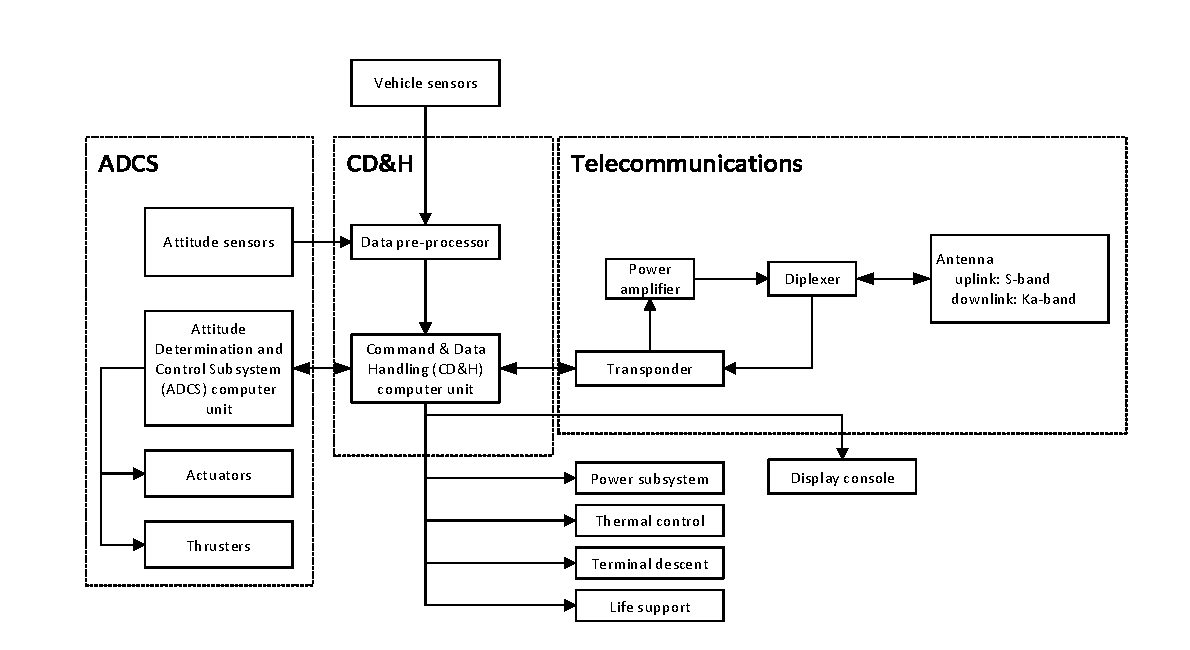
\includegraphics[width=0.95\textwidth]{./Figure/CrewModule/CDH.pdf}
		\caption{Communication flow}
		\label{fig:cdhflow}
\end{figure}

Data processing is performed as follows. Data is first filtered, then analysed to see if reactions are required and in case reactions are required put through to the relevant effectors (subsystems) and critical system information communicated to the ground station via the Ka-band (see section \ref{sec:groundop}). Modulation is performed in the transponder by \gls{bpsk} on the carrier and subcarrier (modulating the carrier) and \gls{qpsk} on the carrier, similar to the Mars Reconnaissance Orbiter mission \cite{Taylor2006}.

For its integral part, it is key that the system is redundantly equipped to ensure adequate system reliability. To this end, cabling is redundant and safety-critical processing tasks are performed by self-checking pair processors, following their application in Orion \cite{Eger2008}. These self-checking pair processors observe and compare the activity of their partner to identify faulty behaviour. 

Antennas used can be extracted from a reference mission to Mars, for example the Mars Reconnaissance Orbiter \cite{Taylor2006}. This mission had relatively high scientific return communications and used a $3$ [$m$] diameter high gain antenna and two low gain antennas. The communication system for this mission was remarkable because it was able to send data back to Earth more than ten times faster than previously conducted missions. Such a high return would be highly beneficial for the manned mission at hand to maximize ground surveillance possibilities and accurate monitoring. It similarly used Ka-band communication for downlink. To this end, the communication system is deemed a good reference system for use in the mission at hand.

The mass of the \gls{cdh} subsystem is extrapolated from that in the Mars Odyssey mission by scaling with the ratio of masses. For a $11.1$ [$kg$] \gls{cdh} subsystem mass in the 376 [$kg$] Mars Odyssey\footnote{URL:\url{http://mars.nasa.gov/odyssey/mission/spacecraft/parts/command/}. Accessed: 11-06-2015}, this translates to nearly $300$ [$kg$] on the $10,000$ [$kg$] entry vehicle at hand. This telecommunications system had a mass of $108$ [$kg$], which is not scaled since the sizing thereof is not deemed mass-dependent. Taking into account a contingency for the larger crew module and more demanding mission at hand as well as the roughness of the estimates, the \gls{cdh} and telecommunications mass is estimated at $530$ [$kg$], thus taking a $30$ $\%$ contingency into account. In addition, cabling requires additional contingency, taken to be $10$ $\%$ and a mass of $53$ [$kg$].


\subsubsection{Operational items} \label{subsec:crewop}
In this section the operational items are sized. This can be summarised as the mass needed by the astronauts to stay alive in the crew module during the mission. For this purpose the paper by Tito et al \cite{tito2013} has been used. In this paper the operational items are called \textcolor{red}{GLS} Environmental Control and Life Support System (ECLSS). First the method for estimation is described with its assumptions. Followed by the results of the estimation.

\paragraph{Estimation method}
\label{par:operationalest}
The mass of the \textcolor{red}{ECLSS (GLS)} is primarily driven by the crew size and mission length. The \textcolor{red}{ECLSS (GLS)} is divided into subsystems: Air Management, Thermal and Humidity Management, Water Management, Waste Management, Human Accommodation, Food Preparation and Storage. Each of these subsystems can be subdivided into components. Examples of these are a water heater or packed food in the Food Preparation and Storage. It is evident that some components scale with the keydrivers and others do not. For example, adding a crew member does not necessitate an extra water heater, but it does require extra packed food. 


Taking this into account the mass has been divided into two components. A basic system mass which scales with crew size and the consumable mass that scales with crew size and mission length.





afasasfasf
\paragraph{Results}
By using the methods from section \ref{par:operationalest} the results of table \ref{tab:operationalest} were obtained.
The masses associated with operational items can be split up into two sections: Basic system mass and consumables mass. Basic system mass consists of the systems concerning crew well-being and life support, such as: Oxygen scrubbers (not including oxygen), atmospheric control systems and food preparation systems. Consumables mass is concerned with items such as oxygen, food, water and personal provisions.
\begin{table}[h]
	\centering
	\caption{Obtained masses and volumes of basic system \& consumable items}
	\begin{tabular}{|p{2cm}|p{2cm}|p{2cm}|p{2.5cm}|p{2.5cm}|}
		\hline
		\textbf{Crew members} & \textbf{Basic system mass $[kg]$} & \textbf{Basic system volume $[m^{3}]$} & \textbf{Consumables mass per day $[kg]$} & \textbf{Consumables volume per day $[m^{3}]$} \\ \hline \hline
		1 & 1,800 & 4.88 & 3.2 & 0.018 \\
		2 & 2,500 & 6.78 & 6.4 & 0.036 \\
		3 & 3,200 & 8.68 & 9.6 & 0.054 \\
		\hline
	\end{tabular}
	\label{tab:operationalest}
\end{table}
It can be seen from table \ref{tab:operationalest} that both the basic system and consumables mass scale with the number of crew members. By using linear extrapolation the mass and volume associated with crew members higher than three can be determined. These are shown in table \ref{tab:crewmemberops} for a mission time of $100$ days.\\

\begin{table}[h]
	\caption{Total mass and volume associated with operational items for varying crew numbers}
	\begin{tabular}{|c|c|c|}
		\hline
		\textbf{Crew members} & \textbf{Operational items mass $[kg]$} & \textbf{Operational items volume $[m^{3}]$}\\ \hline \hline
		1 & 2,120 & 6.69\\
		2 & 3,140 & 10.40\\
		3 & 4,160 & 14.11\\
		4 & 5,180 & 17.82\\
		5 & 6,200 & 21.53\\
		6 & 7,220 & 25.24\\ \hline
	\end{tabular}
	\label{tab:crewmemberops}
\end{table}

\subsubsection{Capsule structure} \label{subsec:crewstruc}
The structure of the crew module serves the important function of connection all the individual subsystems of the crew module and moreover connects with the \gls{hiad}. The main scope of the design described in this report lies within this \gls{hiad}. New advances from for example the currently being developed and Orion mission are therefore not considered. The Orion capsule can already be considered state of the art and is in a large amount representative for the crew module design.

A schematic layout as for example also used in the Orion spacecraft\footnote{URL: \url{http://www.spaceflight101.com/orion-spacecraft-overview.html}, Accessed 11 June 2015 }, features a Aluminium grid structure. This structure encloses the pressurised volume inhabited by the astronauts. The grid structure allows for easy attachment of the individual subsystems. Subsystems which require pressurisation, typically those involving the astronauts can be placed within in this shell, whereas the systems that do not require pressurisation are placed on the outside of this shell. A more detailed analysis on where each of these individual subsystems are placed is discussed in Section \ref{sec:crewpackaging}.


A full estimate of the structural mass is only to be provided in later design phases. More detailed structural estimates are typically provided by detailed \gls{cad} models and \gls{fem} models \cite{Wertz2011}. A rough estimate can be provided on the basis of previous reference missions. \gls{nasa}'s Orion mission is again of primary interest as it also features astronauts. Some differences with respect to the structural elements thereof can however be noted:

\begin{itemize}
\item Orion incorporates an integrated heat shield and structure
\item Orion features a backshell, not required for the inflatable aeroshell by its larger deployed diameter
\end{itemize}

In the design at hand the heat shield structure is incorporated in the \gls{hiad}. The crew module is merely connected to this \gls{hiad} of which the latter is designed in more detail in the remaining chapters of this report. Due to the implementations of the \gls{hiad} a additional backshell structure is also no longer required. The back shell normally functions a protection against thermal loading which moves sideways along the body. Using the large frontal of the inflatable this is prevented, denoting one of the advantages of using a inflatable structure \cite{Hughes2005}. The crew module structure should however also be sized considering , and may as such not be too tall and may feature a tapered end such that the crew module is not exposed to thermal loading passing the \gls{hiad}.

For this reason the heat shield carrier structure of around $1500 \left[kg\right]$ \cite{Ainsworth2014} is not taken into account into the mass estimate of the structure. A total structural mass for manned re-entry vehicles lies at around 30\%. The manned Apollo mission featured a 31\% structural mass fraction \footnote{URL: \url{http://braeunig.us/space/specs/apollo.htm}, Accessed 11 June 2015} including a heat shield structure. Extrapolating this value, with a $9000 \left[kg\right]$ crew module mass yields a structural mass of $1300 \left[kg\right]$, excluding the heat shield structure. This is in line with values suggested by Wertz et al. \cite{Wertz2011}. Taking into account a 30\% mass contingency factor yields a final structural mass estimate of around $1700 \left[kg\right]$. A similar mission featuring a descent towards Mars from $7 \left[km \cdot s^{-1}\right]$ has a structural mass of $517 \left[kg\right]$ on a dry mass of $2863 \left[kg\right]$ including contingency factors\footnote{URL: \url{http://www.nasa.gov/pdf/458812main\_FTD\_AerocaptureEntryDescentAndLanding.pdf} , Accessed 11 June 2015 }. Scaling this value yields a similar mass estimate of around $1800 \left[kg\right]$. 

The connection between the crew module and the \gls{hiad} is taken into account in the capsule structural mass estimate of $1300 \left[kg\right]$.

\subsubsection{Capsule thermal control} \label{subsec:crewthermalcontrol}
Where the \acrfull{tps} is used to protect the crew module from excessive heating during re-entry, the \acrfull{tcs} is used to keep other subsystems in the crew module within their operating temperature limits. It is assumed that re-entry phase does not impose extra requirements on the \gls{tcs} as it is completely covered by the \gls{tps}. Note that this only holds when the angle of attack ($\alpha$) is low enough such that the crew module stays out of the wake. Furthermore, the paper used in the mass estimation for the operational items already assigns a mass for the thermal control withiasd


startracker -30,+50. 

asd



\subsubsection{Capsule power} \label{subsec:pwer}
In order to succefully operate the mission during transfer and the \gls{edl} phase. \\

Piece on the items that the power subsystem needs to drive.\\

Small trade-off / considering possible options for power generation. (solar arrays, batteries, reactor)\\

Power during EDL.\\

conclusion on mass and volume.\\







\subsubsection{Terminal descent system} \label{subsec:crewtermdescent}
Terminal descent takes place in the following sequence:
\begin{enumerate}
\item [HEAT SHIELD EJECTION]
\item At this altitude, retropropulsion is activated and the thruster provides the decelerating force in combination with the inflated aeroshell.
\item At an altitude of 50 [$m$], struts are partially deployed from their stowed position such that the pads rest above the inflatable. At the same time, the vent in the inflation system is opened and inflatable bladders deflate. Upon full deflation, measured by pressure transducers in the inflation system, the struts deploy further such that the pads are level with but below the thruster nozzle exit and achieve a roughly 90 [$deg$] inflatable half-cone angle.
\item The thruster is then deactivated and the crew capsule lands on the inflatable, on which the landing gear pads rest.
\end{enumerate}
Retropropulsion is used for the beneficial aerodynamic interaction with a \gls{hiad} \cite{xxx}, effecting a required specific impulse that is twice as low as otherwise. This effects a smaller propellant mass required. The inflatable is not rejected, but rather deflated, because rejection would require a separation mechanism to prevent interference with the crew capsule. Deflation does induce, however, the risk that it is not performed reliably. In such a case, a risk mitigation plan could be deliberate puncturing of the inflatable bladder volumes in order to deflate it.

[THRUSTER MASS]


The terminal descent system, as described in Section \ref{sec:terminal}, consists of the thruster system that decelerates the spacecraft from Mach 5 at 10 [km] height to zero velocity at a height of 0 [km]. The thruster should be placed in the centerbody and pointed in the forward direction, such that the positive interaction between aerodynamics and the thruster plume is made use of. The total thruster mass, including fuel is estimated to be approximately 1300 [kg], based on extrapolation of .................
The thruster mass is estimated to be 470 [kg], based on a 3g deceleration and using an empirical relation\cite{Christian2006}. This leaves approximately 930 [kg] for the fuel. Assuming the density of the fuel at 1000 $[kg\cdot m^{-3}]$\footnote{\url{http://en.wikipedia.org/wiki/Liquid-propellant_rocket}. Accessed: 11-06-2015} means the required volume for fuel is 0.93 [$m^3$].






\subsection{Crew module configuration} \label{sec:crewpackaging}
Space allocation of the subsystems described in the previous section, as well as crew members, is performed with the goals of:
\begin{itemize}
\item Accommodating subsystems necessary to support interplanetary flight and entry
\item Providing crew members with a habitable volume and operational items to support a flight duration of approximately 100 days
\item Keeping the axial position of the \gls{cg} forward to lower pitch stability and alleviate pitch control performance in the final mission phase
\item Allowing for packaging freedom in achieving a static lateral \gls{cg} offset for creating an asymmetric lifting shape
\end{itemize}
To this end, the crew module is packaged as depicted in Figures \ref{fig:axview} and \ref{fig:topview}. 

The top part is required to contain drogues to stabilize the entry vehicle in its final descent phase. Four drogues are placed to incorporate redundancy and provide
a symmetric configuration, to prevent excessive tilting during final descent. Moreover, the top part contains the foldable solar arrays required to generate power required during interplanetary transfer. These are placed in the top part to prevent interference with the flow during entry on one hand and with thrusters and the stowed inflatable before entry on the other hand. A high-gain antenna of adjustable attitude on a boom enables communication during all mission phases. A first-order estimate for the length of this upper part is $0.2$ $[m]$, based on the Orion configuration\footnote{URL:\url{http://www.spaceflight101.com/orion-spacecraft-overview.html}. Accessed: 15-06-2015}.

Crew members are located in the next part, a habitable volume to their availability that is dictated by the performance limit for a three-month mission duration as 11 $[m^{3}]$ per crew member \cite{Rudisill2008}. The diameter of the habitable volume is 4.0 $[m]$, thereby less than vehicle maximum diameter to accommodate four propellant tanks, one per quadrant, that allow intertank propellant transfer to shift the lateral \gls{cg} position. The tanks are sized on the basis of the total required propellant and provide propellant for both the reaction control thrusters and main thruster. The length of this part follows from the habitable volume and depends on the number of crew members.

Operational items are located below, within reach of crew members. These are placed at this location because of their relatively high mass and therefore contribution to the axial \gls{cg} position. The total volume occupied follows from Table \ref{tab:crewmemberops}. On one hand these operational items include relatively dense products, foremostly the life support systems, and less dense products in the form of food and other supplies. Arranging these items asymmetrically allows for a lateral \gls{cg} offset, most notably considering the depleted supplies of food at the end of interplanetary transfer while life support system mass remains intact. The length of this part follows from the required volume for operational items.

The last part of the crew module contains four struts for touchdown, packed symmetrically. The struts are arranged about the batteries required to provide power during entry, where solar panels are stowed, a nitrogen tank for inflation of the inflatable aeroshell and the main thruster to provide in-plane velocity changes. The length follows from estimates for the strut required volume based on the Apollo landers and is an estimated 1.0 $[m]$. 

The last part contains the thruster nozzle, closed off by a heat-resistant end-cap during entry, and the attachment rings for the inflatable decelerator. It is detachable from the main body and thereby does not contain any other subsystems. The length of this part is mainly dictated by the shape of the inflatable and where it attaches to the centerbody.

\begin{figure}[h]
		\centering
		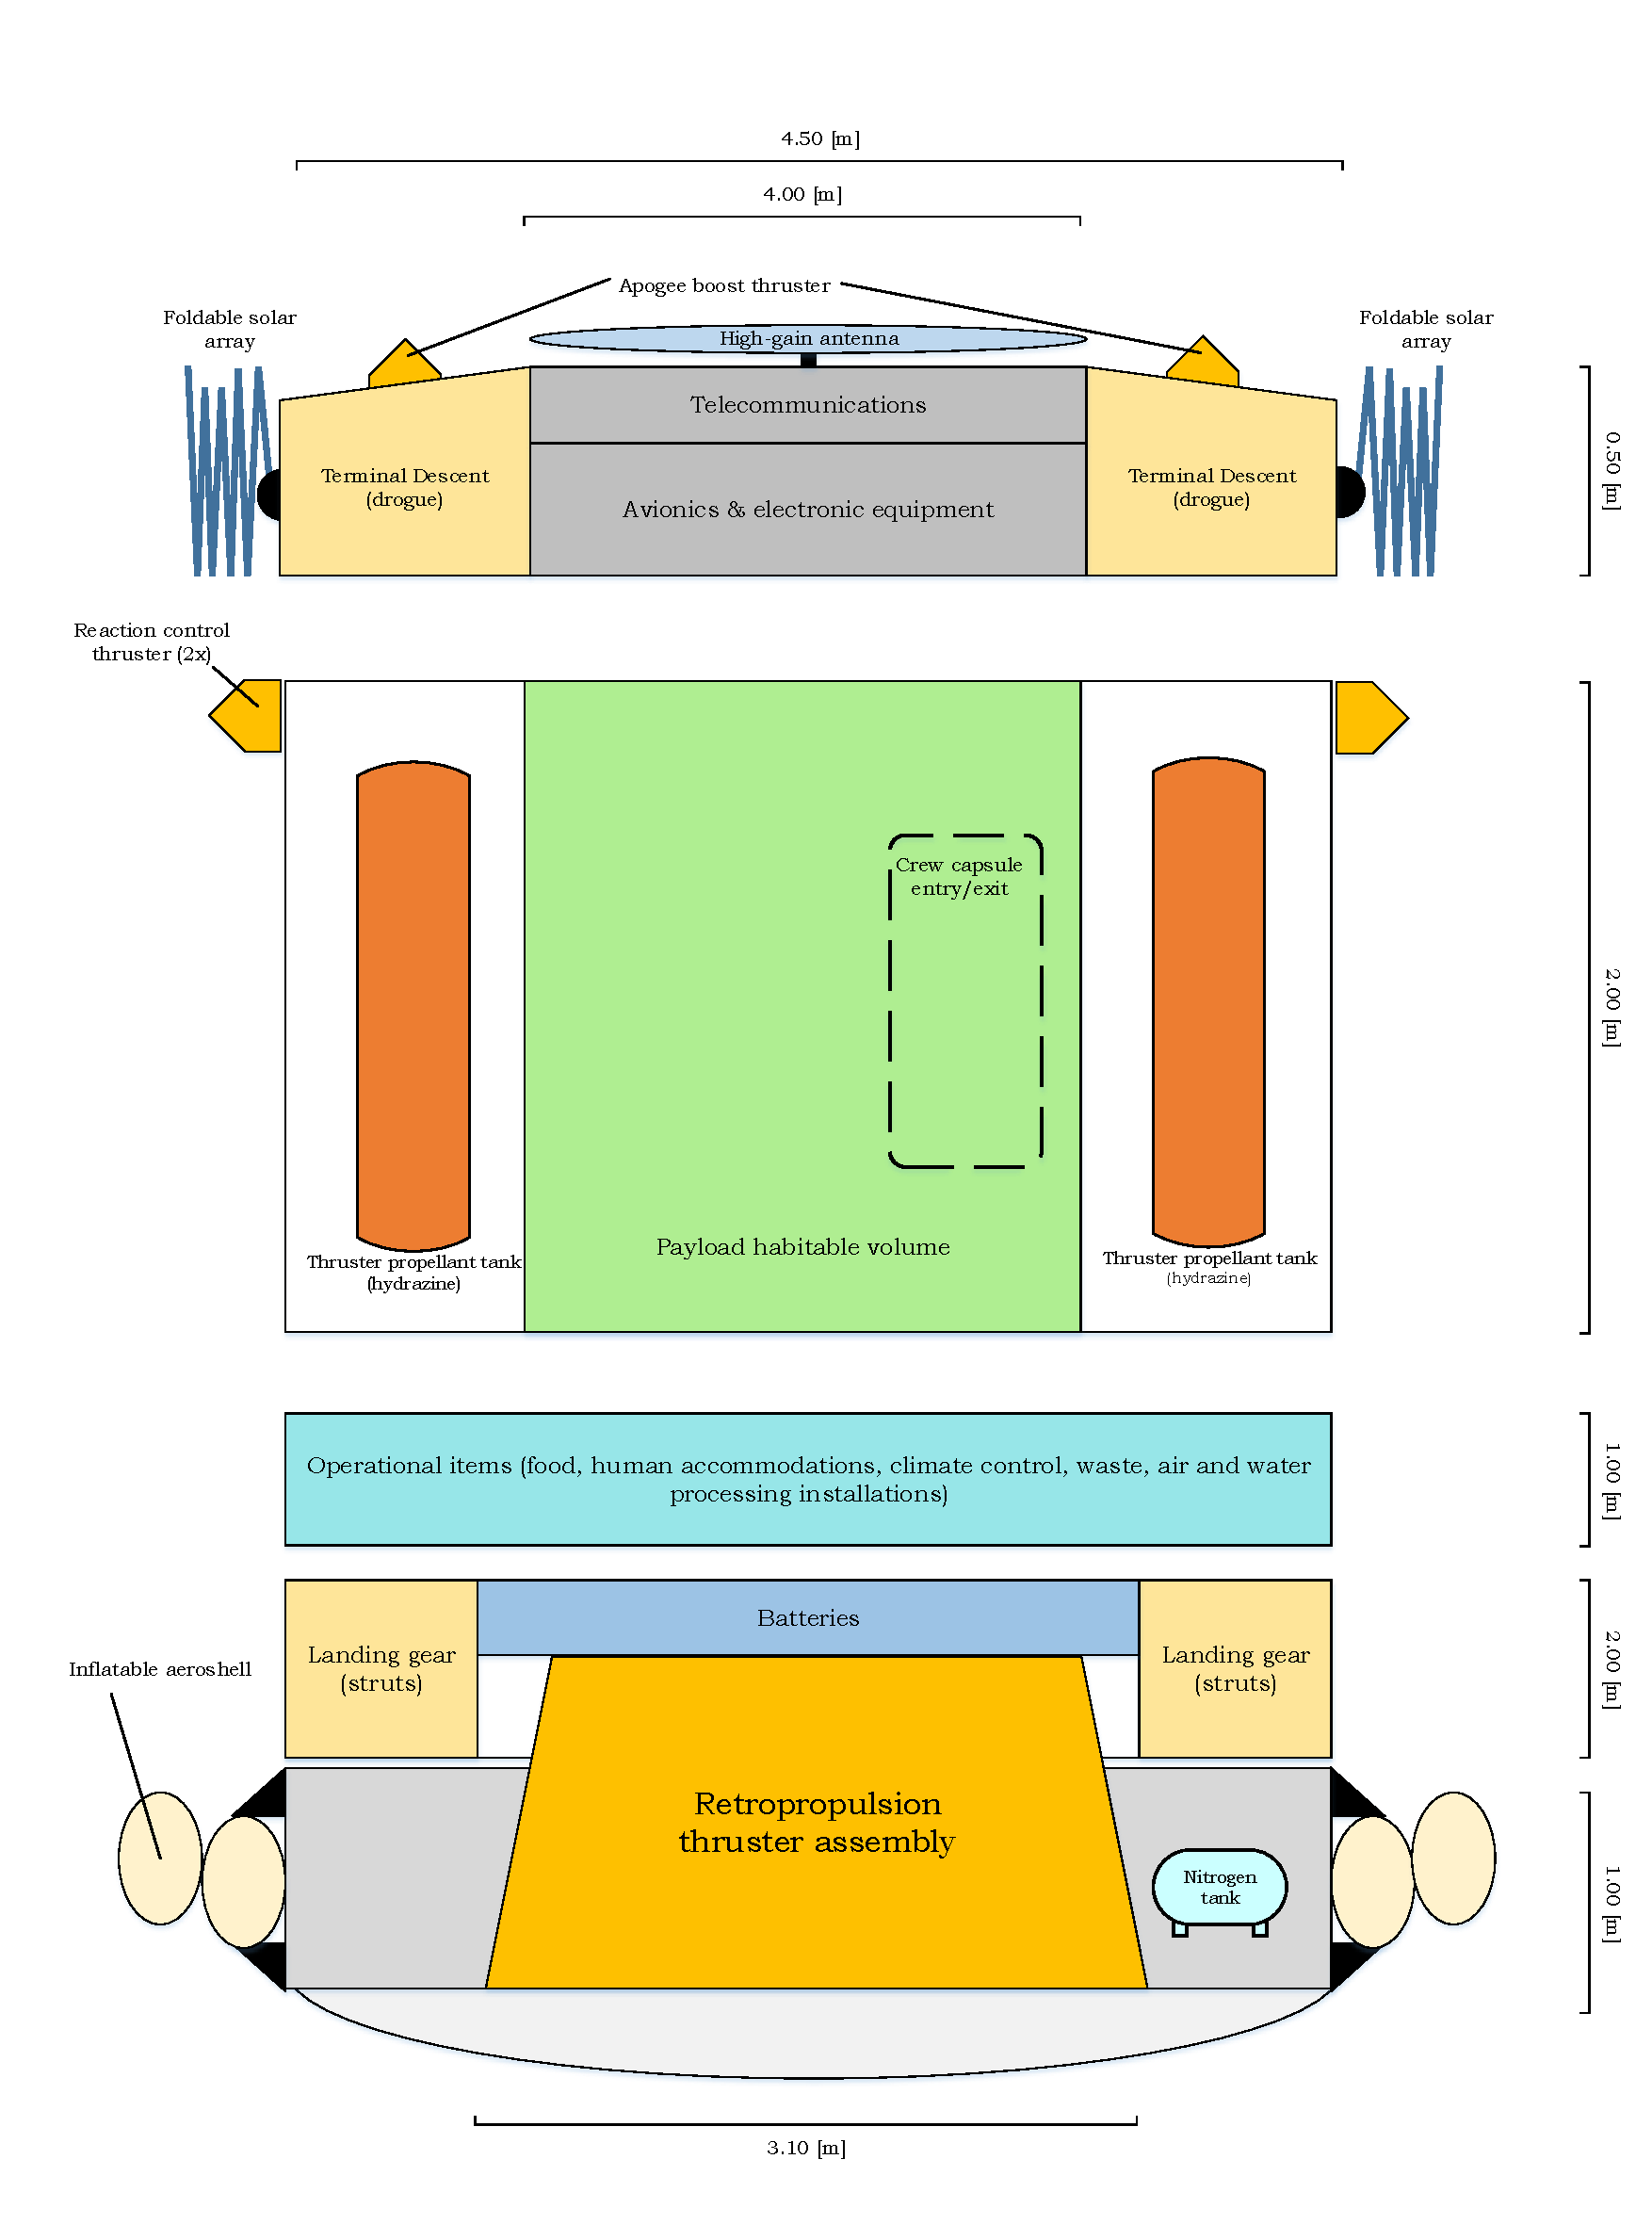
\includegraphics[width=0.95\textwidth]{./Figure/CrewModule/Axialview.pdf}
		\caption{Axial view of crew module lay-out}
		\label{fig:axview}
\end{figure}

\begin{figure}[h]
		\centering
		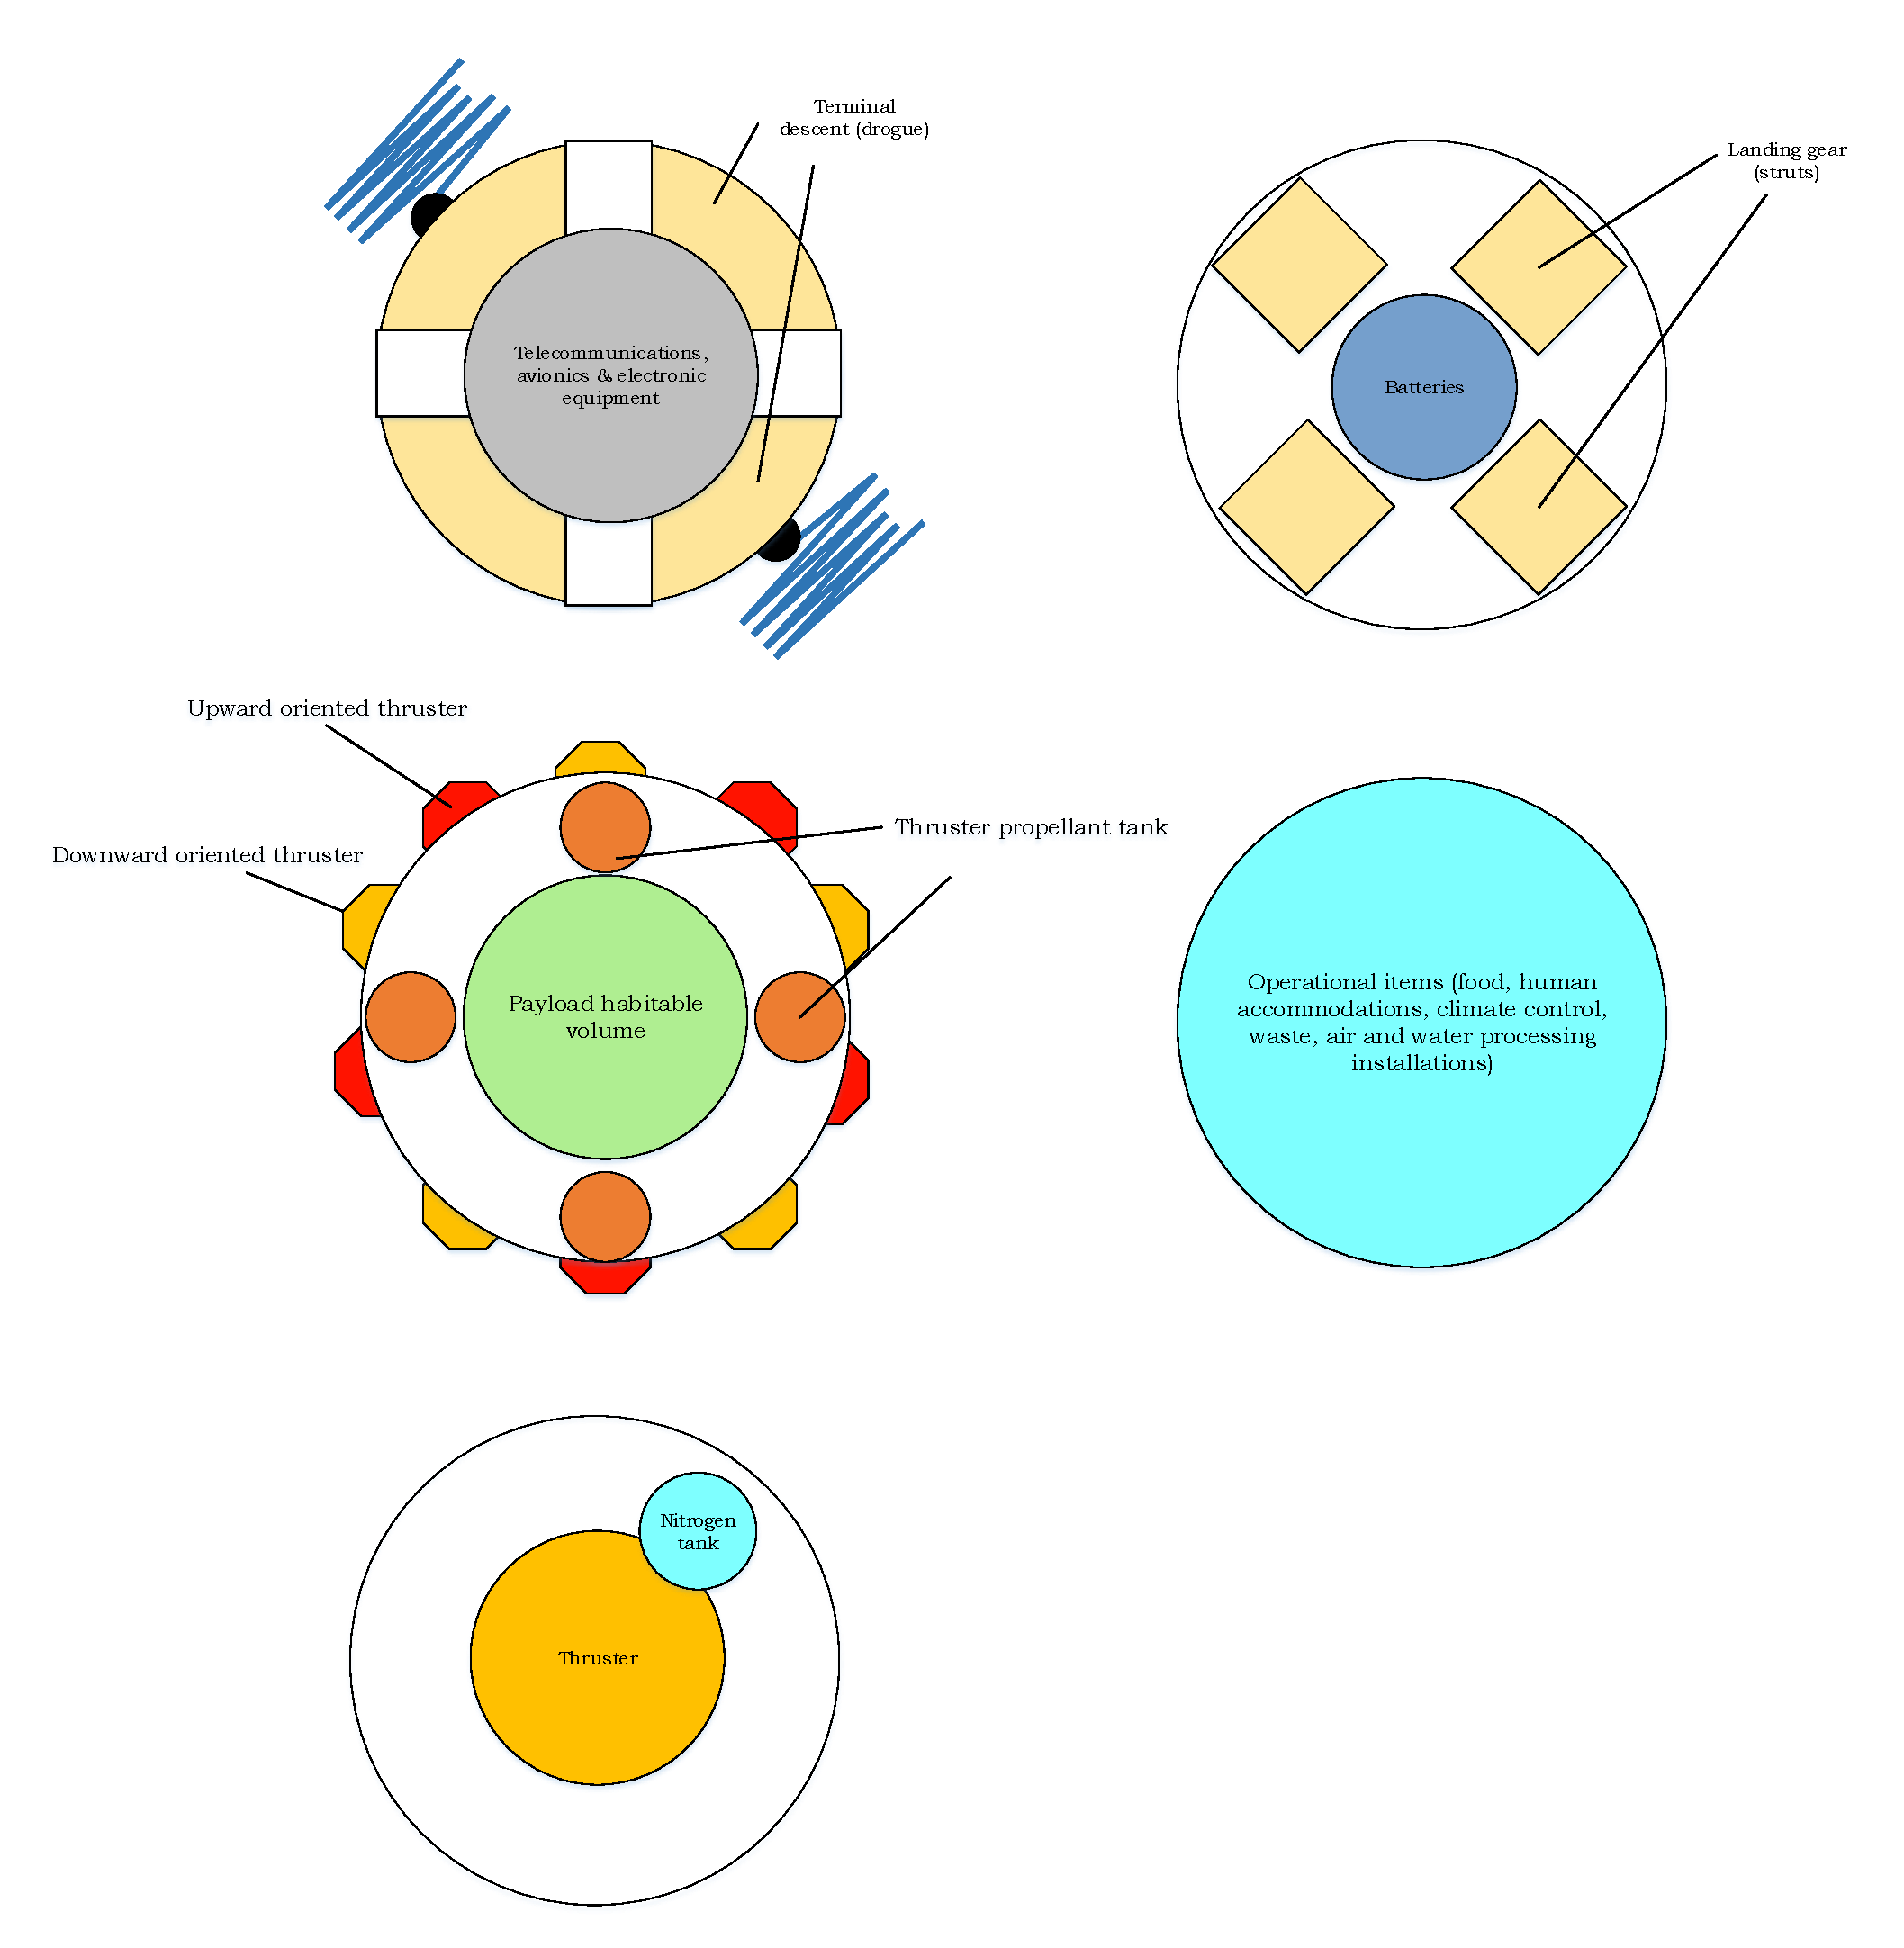
\includegraphics[width=0.95\textwidth]{./Figure/CrewModule/TopviewV2.pdf}
		\caption{Top-down view of crew module lay-out}
		\label{fig:topview}
\end{figure}




